\documentclass[]{beamer}
% Class options include: notes, notesonly, handout, trans,
%                        hidesubsections, shadesubsections,
%                        inrow, blue, red, grey, brown

% Theme for beamer presentation.
\usepackage{beamerthemesplit} 
% Other themes include: beamerthemebars, beamerthemelined, 
%                       beamerthemetree, beamerthemetreebars  

\graphicspath{ {../../figures/} }


\title{Robustness in White Rabbit}    % Enter your title between curly braces
\author{Maciej Lipinski, Cesar Prados} % Enter your name between curly braces
\institute{CERN \&  GSI}      % Enter your institute name between curly braces
\date{14/04/2011}             % Enter the date or \today between curly braces

\usepackage{graphicx}
\usepackage{epstopdf}

\begin{document}

% Creates title page of slide show using above information
\begin{frame}
  \titlepage{}
\end{frame}
\note{Talk for 30 minutes} % Add notes to yourself that will be displayed when
                           % typeset with the notes or notesonly class options

%%%%%%%%%%%%%%%%%%%%%%%%%%%%%%%%%%%%%%%%%%%%%%%%%%%%%%%%%%%%%%%%%%%%%%%%%%%%%%%
\section*{Outline}
%%%%%%%%%%%%%%%%%%%%%%%%%%%%%%%%%%%%%%%%%%%%%%%%%%%%%%%%%%%%%%%%%%%%%%%%%%%%%%%
\begin{frame}
  \tableofcontents
\end{frame}
%%%%%%%%%%%%%%%%%%%%%%%%%%%%%%%%%%%%%%%%%%%%%%%%%%%%%%%%%%%%%%%%%%%%%%%%%%%%%%%
\section{Robustness}
%%%%%%%%%%%%%%%%%%%%%%%%%%%%%%%%%%%%%%%%%%%%%%%%%%%%%%%%%%%%%%%%%%%%%%%%%%%%%%%
\subsection{What is a robust White Rabbit Network}
\begin{frame}
  \frametitle{Definition}
%%%%%%%%%%%%%%%%%%%%%%%%%%%%%%%%%%%%%%%%%%%%%%%%%%%%%%%%%%%%%%%%%%%%%%%%%%%%%%%
\centering

A White Rabbit Network (WRN) is considered robust only if all the WR nodes
connected to the network always receive data on time and are always
synchronized with the required accuracy. The amount of lost frames in a given 
period of time never exceeds the upper bound.

\end{frame}

%%%%%%%%%%%%%%%%%%%%%%%%%%%%%%%%%%%%%%%%%%%%%%%%%%%%%%%%%%%%%%%%%%%%%%%%%%%%%%%
\subsection{Naming Conventions}
\begin{frame}
  \frametitle{Naming Conventions}
%%%%%%%%%%%%%%%%%%%%%%%%%%%%%%%%%%%%%%%%%%%%%%%%%%%%%%%%%%%%%%%%%%%%%%%%%%%%%%%
\centering

\begin{itemize}
  \item Granularity Window (GW).
  \item Types of the information distributed over WRN:
  \begin{itemize}
    \item Control Data - Control Messages (CM),
    \item Clock        - timing information (PTP+SyncE),
    \item Standard Data - all the other Ethernet traffic,
  \end{itemize}
  \item Class of Service and Quality of Service (CoS and QoS),
  \item High Priority traffic (HP),
  \item Standard Priority traffic (SP).
\end{itemize}

\textcolor{red}{DISCUSSION:} \\
Most of the names introduced here are not in line with standard naming
conventions and need to be changed, ideas appreciated.

\end{frame}

%%%%%%%%%%%%%%%%%%%%%%%%%%%%%%%%%%%%%%%%%%%%%%%%%%%%%%%%%%%%%%%%%%%%%%%%%%%%%%%
\subsection{Areas of Consideration}
\begin{frame}
  \frametitle{Areas of Consideration}
%%%%%%%%%%%%%%%%%%%%%%%%%%%%%%%%%%%%%%%%%%%%%%%%%%%%%%%%%%%%%%%%%%%%%%%%%%%%%%


\begin{itemize}
  \item Determinism
  \item Clock Resilience
  \item Data Resilience
  \item Monitoring and Diagnostics
\end{itemize}

\end{frame}

%%%%%%%%%%%%%%%%%%%%%%%%%%%%%%%%%%%%%%%%%%%%%%%%%%%%%%%%%%%%%%%%%%%%%%%%%%%%%%%
\subsection{Requirements}
\begin{frame}
  \frametitle{Requirements}
%%%%%%%%%%%%%%%%%%%%%%%%%%%%%%%%%%%%%%%%%%%%%%%%%%%%%%%%%%%%%%%%%%%%%%%%%%%%%%

\begin{table}[ht]
\centering
	\begin{tabular}{| c | c | c |}          \hline
\textbf{Requirement     }& \multicolumn{2}{|c|}{\textbf{Value(s)}}  \\
                         & GSI              & CERN          \\ \hline
Granuality Window        & 100$\mu s$       & 1000$\mu s$   \\ \hline
Maximum Link Length      & 2km              & 10km          \\ \hline
Control Message Size     & 200-500 bytes    & 1200 - 5000 bytes     \\ \hline
Synchronization accuracy & probably 8ns     & most nodes 1$\mu s$ \\
                         &                  & few nodes  ~2ns \\ \hline
Control Message loss rate&  ?               & ?                  \\ \hline

\end{tabular}
\label{tab:requirements}
\end{table}

\centering
\textcolor{red}{DISCUSSION:}\\
What is the real-life requirement for number of CM lost per year?\\
GW of 100$\mu s$ is very tight and needs solid justification.

\end{frame}

%%%%%%%%%%%%%%%%%%%%%%%%%%%%%%%%%%%%%%%%%%%%%%%%%%%%%%%%%%%%%%%%%%%%%%%%%%%%%%
\section{Areas of Consideration}
\subsection{Determinism}
%%%%%%%%%%%%%%%%%%%%%%%%%%%%%%%%%%%%%%%%%%%%%%%%%%%%%%%%%%%%%%%%%%%%%%%%%%%%%%
\begin{frame}
  \frametitle{Delivery Delay Estimation}   


  \begin{columns}[c]
  \column{2.5in}  % slides are 3in high by 5in wide
  \begin{itemize}
  \item Control Message of 500 Bytes is encoded with FEC into 4 Ethernet frames
        of $\approx375$ Bytes \textcolor{blue}{(current FEC 4x288 Bytes)}
  \item Store-and-Forward implemented in SWCore is not sufficient for GSI's GW
        (100$us$).
  \end{itemize}

  {\tiny
  \begin{table}[ht]
  \centering
	  \begin{tabular}{| c | c | c | c |}          \hline
  \textbf{CM size}& \multicolumn{2}{|c|}{\textbf{CM Delivery Delay}}\\
		 &    GSI           & CERN          \\ \hline
  200 bytes      &  92.2$\mu s$    & 132.2$\mu s$    \\ \hline
  500 bytes      & 228.7$\mu s$    & 268.3$\mu s$    \\ \hline
  1500 bytes     & 272.2$\mu s$    & 312.2$\mu s$    \\ \hline
  5000 bytes     & 349.3$\mu s$    & 389.3$\mu s$    \\ \hline
  \end{tabular}
  \label{tab:CMspDelay}
  \end{table}
 }

  \column{3in}

  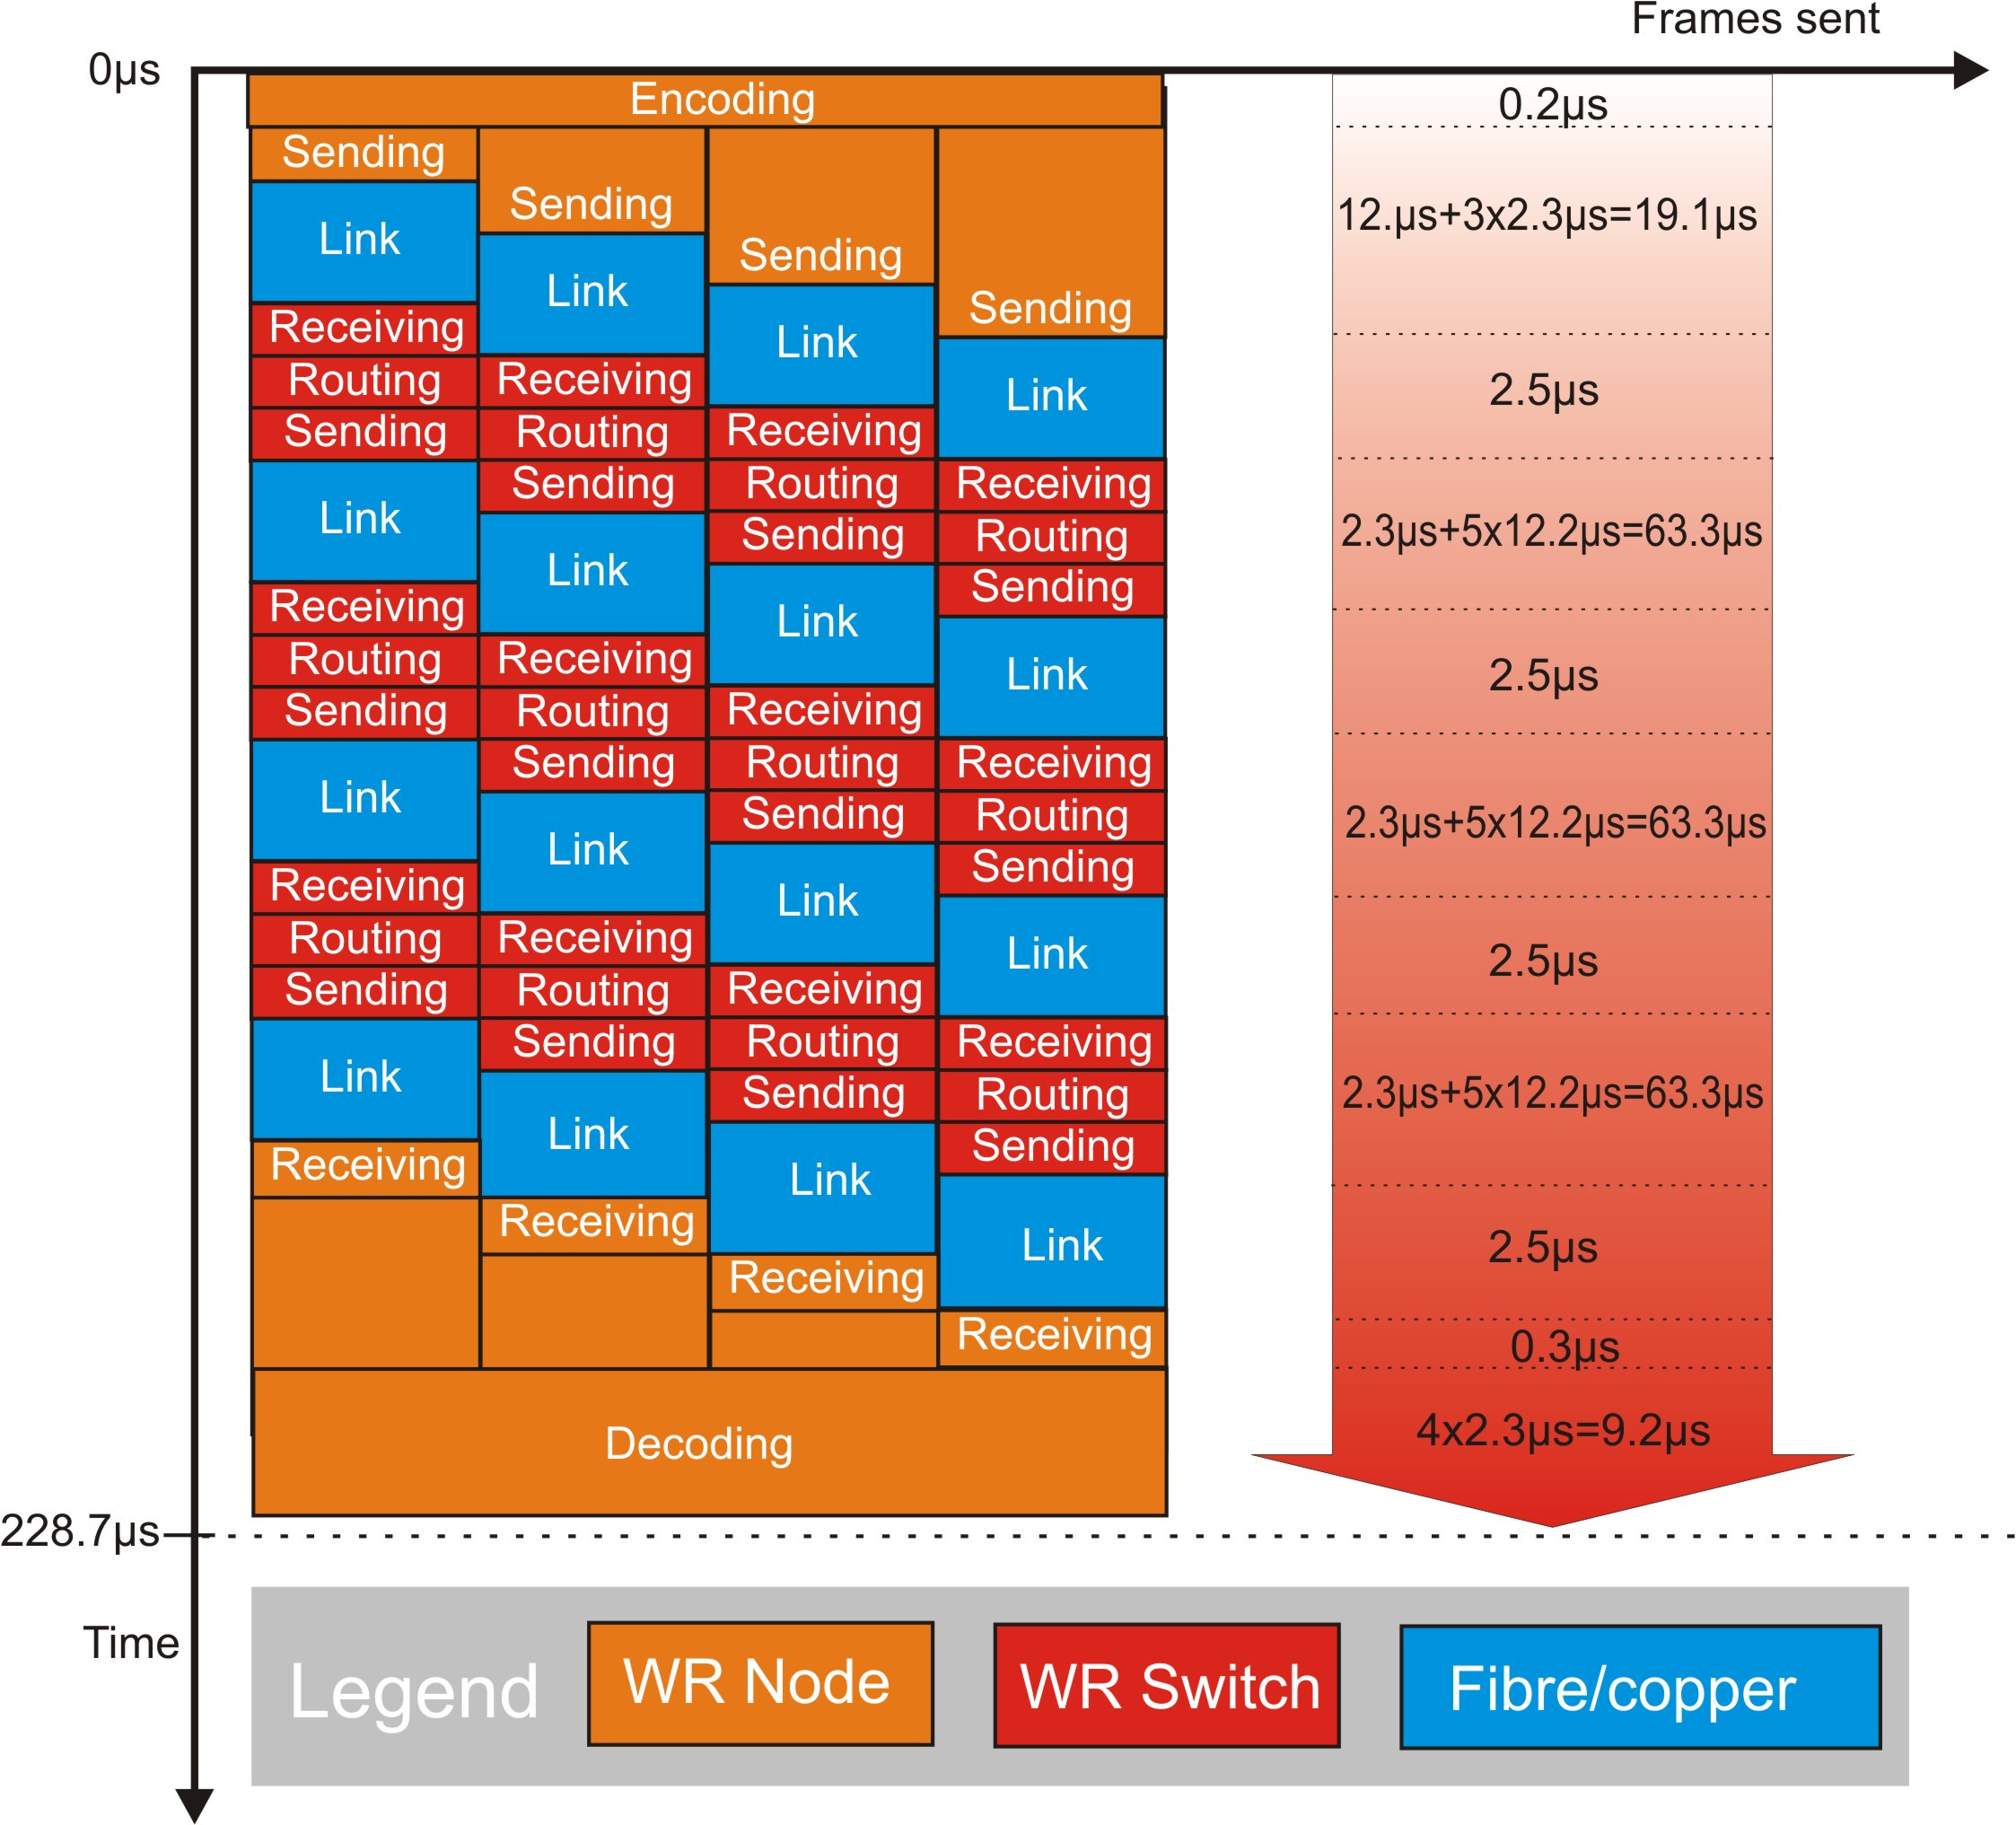
\includegraphics[height=5.2cm,keepaspectratio]{robustness/CMdelayStandard.ps}

  \end{columns}



\end{frame}
%%%%%%%%%%%%%%%%%%%%%%%%%%%%%%%%%%%%%%%%%%%%%%%%%%%%%%%%%%%%%%%%%%%%%%%%%%%%%%
% 
\begin{frame}
  \frametitle{Cut-through HP Bypass}
 
  \begin{columns}[c]
  \column{2.8in}  % slides are 3in high by 5in wide
  \begin{itemize}
  \item All the broadcast traffic with priority 7 is cut-through forwarded
        using  HP Bypass.
  \item Ideas concerning HP traffic collisions :
  \begin{itemize}
    \item Single source of HP Traffic.
    \item Priority of HP Traffic from Data Master (DM), drop non-DM on
          collision.
  \end{itemize}
  \end{itemize}
\centering
\textcolor{red}{DISCUSSION:} \\
Drop on collision, sending of HP by more Data Master and/or nodes.

  \column{2.3in}
  \centering
  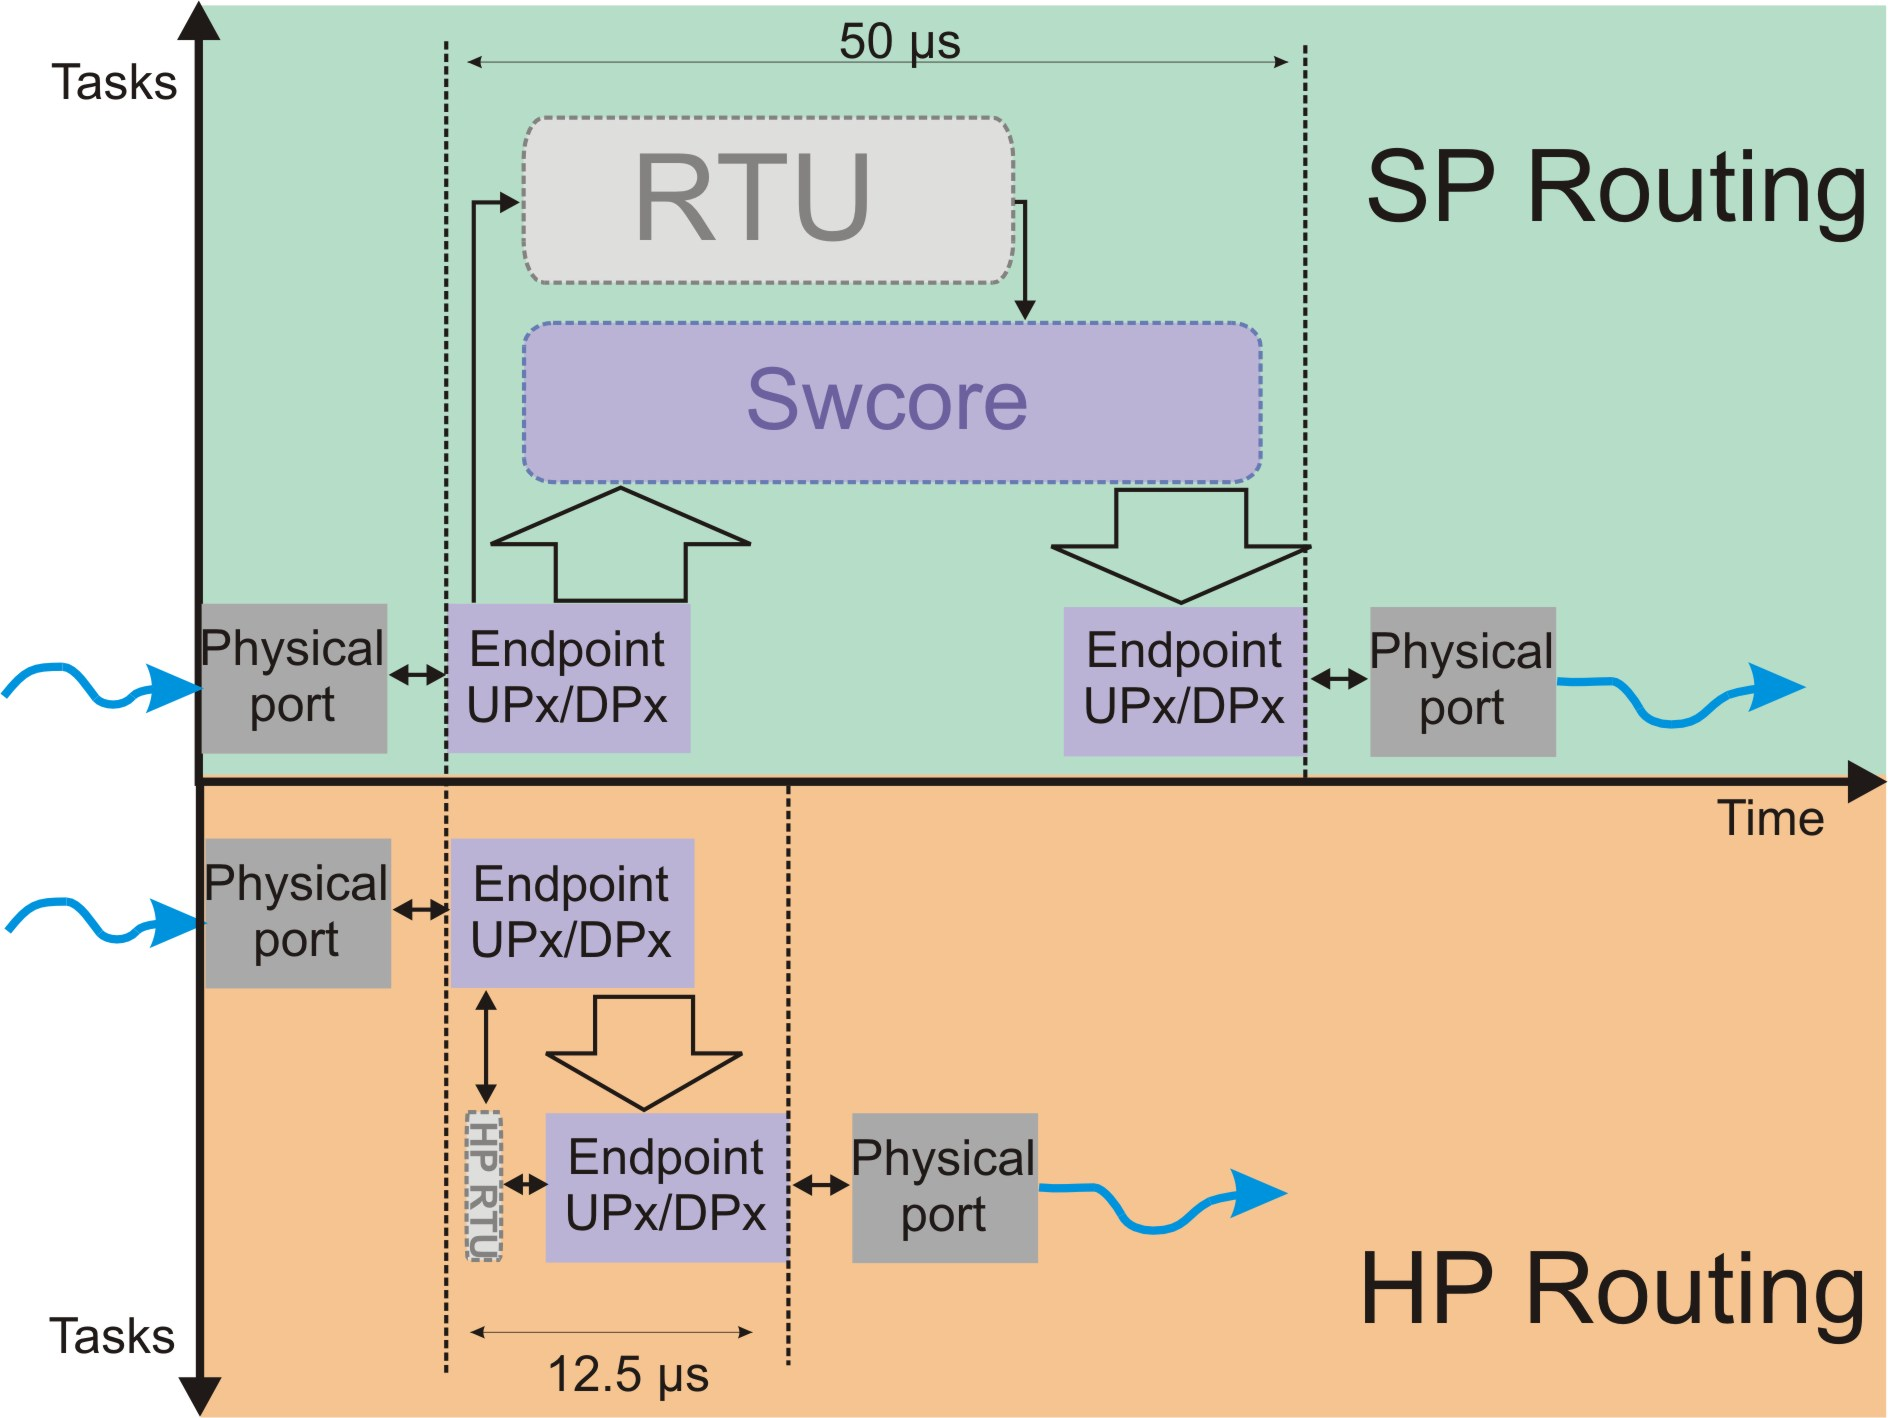
\includegraphics[height=4cm,keepaspectratio]{robustness/SWhpRouting.ps}
  {\tiny
  \begin{table}[ht]
  %\centering
	  \begin{tabular}{| c | c | c | c |}          \hline
  \textbf{CM size}& \multicolumn{2}{|c|}{\textbf{CM Delivery Delay}}\\
		&    GSI           & CERN          \\ \hline
  200 bytes      &  63.2$\mu s$     & 103.2$\mu s$    \\ \hline
  500 bytes      &  76.3$\mu s$     & 116.3$\mu s$    \\ \hline
  1500 bytes     & 106.4$\mu s$     & 146.4$\mu s$    \\ \hline
  5000 bytes     & 175.8$\mu s$     & 215.8$\mu s$    \\ \hline
  \end{tabular}
  \label{tab:CMspDelay}
  \end{table}
  }

  \end{columns}

\end{frame}


%%%%%%%%%%%%%%%%%%%%%%%%%%%%%%%%%%%%%%%%%%%%%%%%%%%%%%%%%%%%%%%%%%%%%%%%%%%%%%
\subsection{Clock Resilience}
\begin{frame}
  \frametitle{Synchronization Stability}   
%%%%%%%%%%%%%%%%%%%%%%%%%%%%%%%%%%%%%%%%%%%%%%%%%%%%%%%%%%%%%%%%%%%%%%%%%%%%%%

\begin{itemize}
  \item Clock Stability preservation during switch-over (change of clock
        source-port).
  \item Two dependencies:
  \begin{itemize}
    \item Syntonization -- SyncE - PLLs by Tomek are designed to accommodate
          many clock sources, theoretically stability during switch-over is not
          an issue.
    \item Synchronization -- WRPTP - Each port speaks independently WRPTP
          unaware which one is active, no change WRPTP-wise during switch over.
  \end{itemize}
 \item Tests are needed to prove the theory in practice.
 \item Logical topology of Clock distribution is aligned with logical topology
       of Data, active and backup ports (clock/data sources) assigned
       using Rapid Spanning Tree Protocol.
\end{itemize}

\end{frame}

%%%%%%%%%%%%%%%%%%%%%%%%%%%%%%%%%%%%%%%%%%%%%%%%%%%%%%%%%%%%%%%%%%%%%%%%%%%%%%
\subsection{Data Resilience}
\begin{frame}
  \frametitle{Probability of WRN failure}   
%%%%%%%%%%%%%%%%%%%%%%%%%%%%%%%%%%%%%%%%%%%%%%%%%%%%%%%%%%%%%%%%%%%%%%%%%%%%%%
{\tiny
\begin{table}[ht]
	\begin{tabular}{| c | c | c |}          \hline
\textbf{Requirement name}& \multicolumn{2}{|c|}{\textbf{Value(s)}}  \\
                         & GSI              & CERN          \\ \hline
max Failure rate ($\lambda_{WRN_{max}}$) & $3.170979198*10^{-12}$ &
$3.170979198*10^{-11}$  \\ \hline
\end{tabular}
\label{tab:requirements}
\end{table}
}


\begin{equation}
  \label{equation:WRreliability}
     P_{WRN_f} =  P_{congestion} + P_{f\_FEC} + P_{f\_Network}
\end{equation}
{\small
\begin{itemize}
        \item $P_{congestion}$ - Control Message lost (dropped) due to congestion.
        \item $P_{f\_FEC}$ - FEC fails to recover Control Message.
        \item $P_{f\_Network}$ - single network component failure. 
\end{itemize}
}
{\tiny
\begin{table}[ht]
\begin{tabular}{|p{2cm}|p{1cm}|p{1cm}|p{1.5cm}|p{1.5cm}|}        \hline
& \textbf{WRS Number} &
\textbf{Nodes MAX Number} &  
\multicolumn{2}{|p{3cm}|}{\textbf{$MTBF_{Switch}$=  20 000[h] }} \\
Topology & & & $P_f$ & MTBF[h]  \\ \hline
%1   &   3   &  14336  &   r1   &   r2   &   r3   &   r4   &   r5    \\ \hline

No-redundant &  127 &  2048  
& $ 2.08*10^{-3}$  & $ 5.77*10^{3}$
 \\ \hline

Double-redundancy &  292 &  2048  
& $ 4.71*10^{-7}$  &  $ 2.55*10^{7}$
   \\ \hline

Triple-redundancy &  495  & 2048    
& $ 3.06*10^{-11}$  &  $ 4.08*10^{11}$
  \\ \hline
\end{tabular}
\end{table}
}

\end{frame}
%%%%%%%%%%%%%%%%%%%%%%%%%%%%%%%%%%%%%%%%%%%%%%%%%%%%%%%%%%%%%%%%%%%%%%%%%%%%%%
%\subsection{Data Resilience}  %!!!!
\begin{frame}
  \frametitle{Topology Redundancy}   
%%%%%%%%%%%%%%%%%%%%%%%%%%%%%%%%%%%%%%%%%%%%%%%%%%%%%%%%%%%%%%%%%%%%%%%%%%%%%%

  \begin{columns}[c]
  \column{3.8in} 

  \begin{itemize}
  \item Increases Clock and Data resilience by eliminating \textit{single point
	of failure} \textcolor{red}{(only if redundant connection to WR Node is
	considered)}.
  \item Enables to achieve reliability of entire network greater then
	reliability of its single component.
  \item First estimations show that double redundancy is not enough to achieve
	reliability of 1 CM lost per year, TO BE confirmed with more studies.
  \item The redundancy of the WRN is justified only if Data Master is
	highly reliable or redundant.
  \end{itemize}

  \column{1.2in}
  \centering
  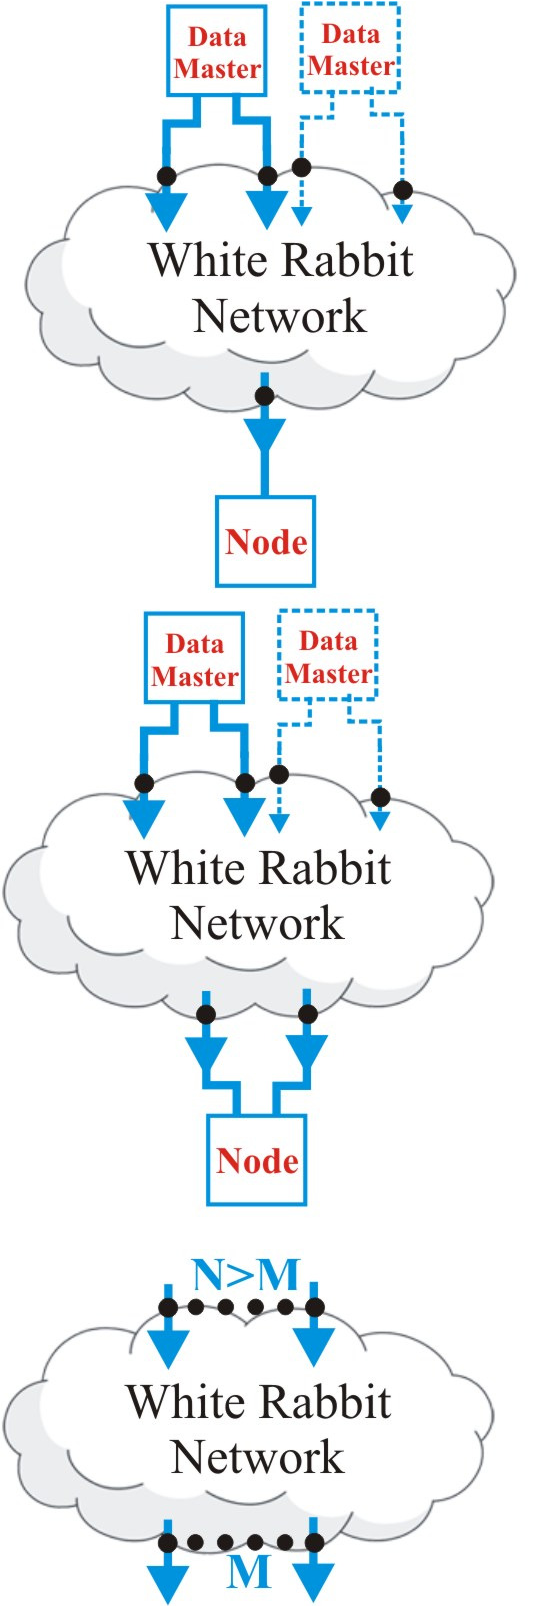
\includegraphics[height=5cm,keepaspectratio]{robustness/inOutOfWRN.ps}

  \end{columns}
\centering
\textcolor{red}{DISCUSSION:} \\
Redundant connection to WR nodes.

\end{frame}
%%%%%%%%%%%%%%%%%%%%%%%%%%%%%%%%%%%%%%%%%%%%%%%%%%%%%%%%%%%%%%%%%%%%%%%%%%%%%%

\begin{frame}
  \frametitle{Triple-redundancy of topology}
  \centering
  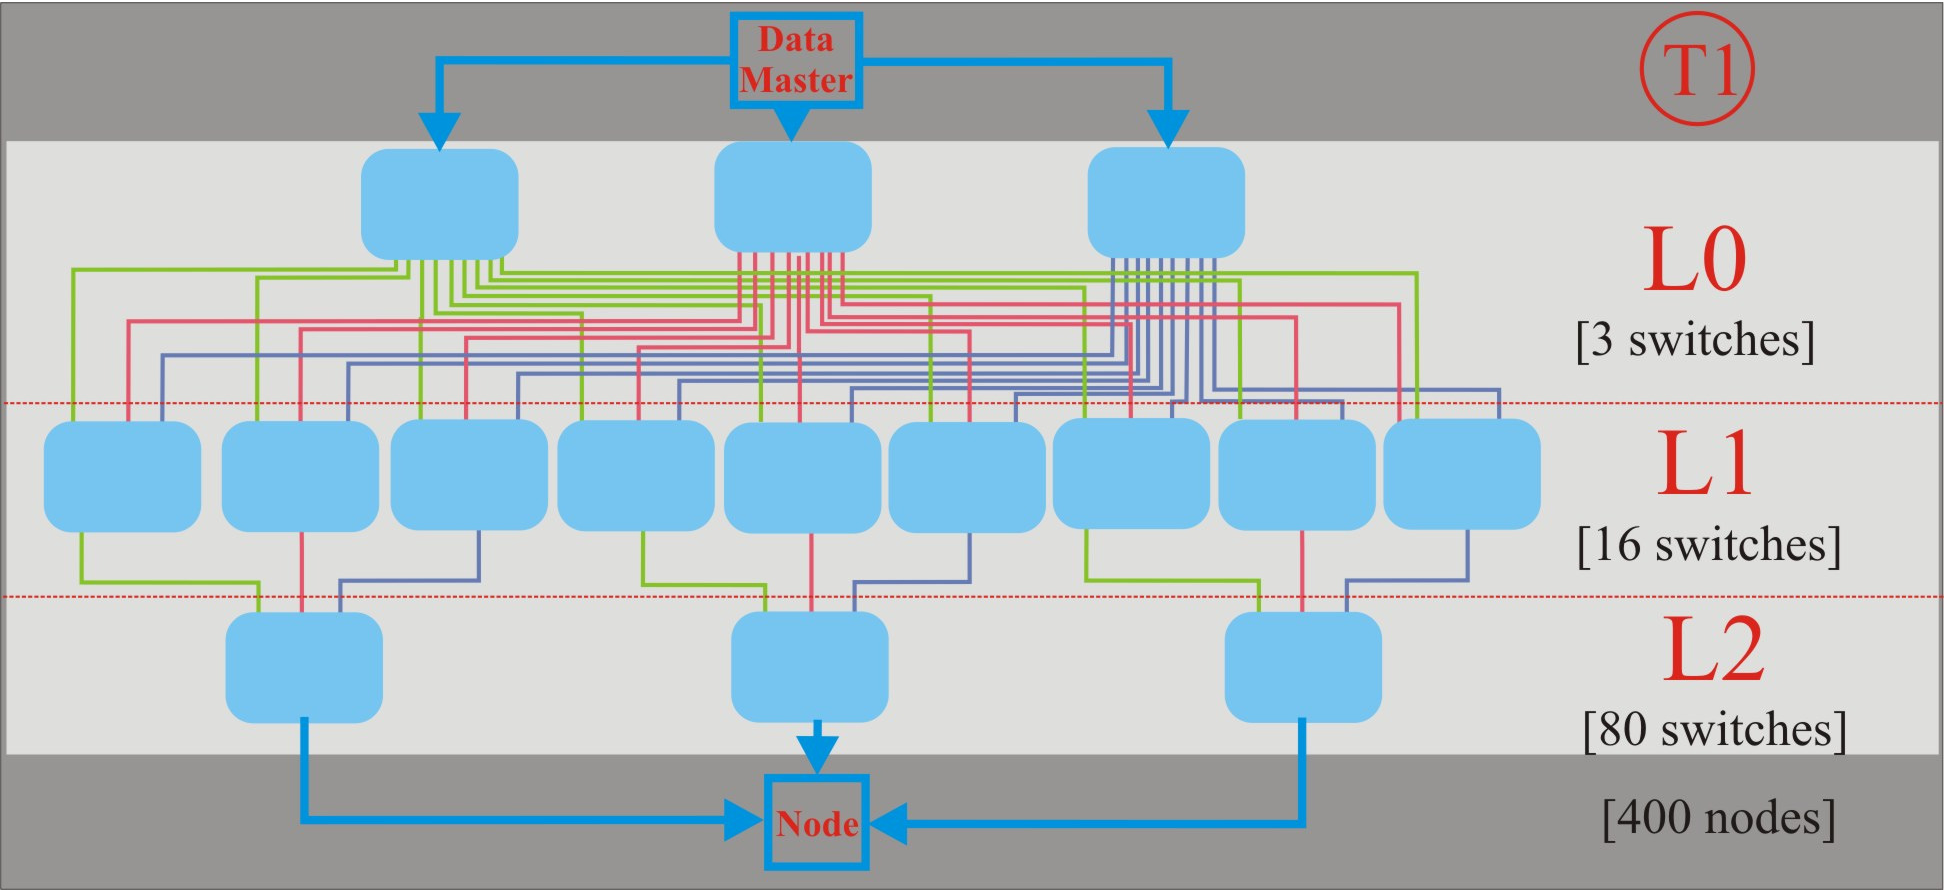
\includegraphics[height=4cm,keepaspectratio]{robustness/tripleTopology}

  \begin{itemize}
  \item For $\approx$2000 WR nodes connected to two layers of switches,
        15 switches in L0, 80 in L1 and 400 in L2 are required (total 495)
  \end{itemize}

\end{frame}
%%%%%%%%%%%%%%%%%%%%%%%%%%%%%%%%%%%%%%%%%%%%%%%%%%%%%%%%%%%%%%%%%%%%%%%%%%%%%%

\begin{frame}
  \frametitle{Rapid Spanning Tree Protocol in WR (WR RSTP)}
  
  \begin{columns}[c]
  \column{3.8in} 

  \begin{itemize}
  \item Requirements:
  \begin{itemize}
    \item Fast switching to alternate/backup link so that not more then 2 HP
          Frames are lost, e.g.: CM of 500 Bytes, FECed into 4 Ethernet frames
          of 288 Bytes, each transmitted 2.3$us$ -- switching time $<$ 2.3$us$
    \item Alternate path length : max 1 hop longer primary path length.
  \end{itemize}
  \item The speed of White Rabbit RSTP is directly associated minimum CM size.
  \item Hardware support for HP traffic (only) using RSTP and restricting
        possible topologies.
  \end{itemize}

  \column{1.2in}

  \centering
  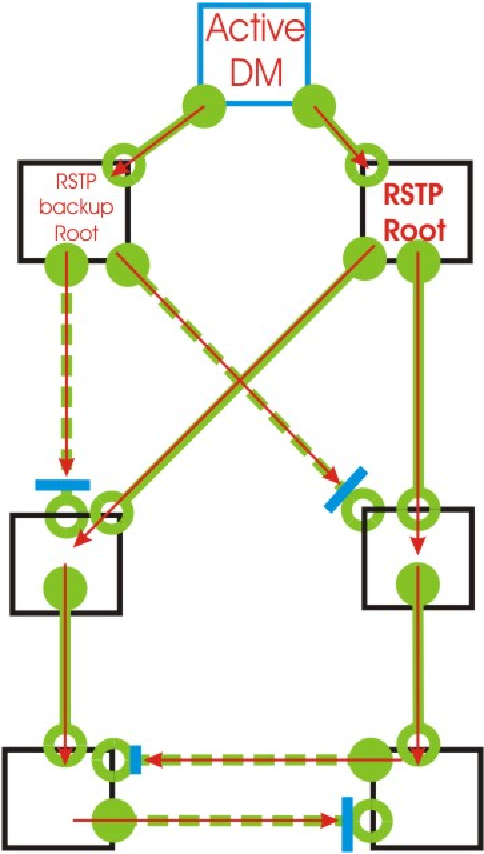
\includegraphics[height=5cm,keepaspectratio]{robustness/RSTPcomplex.ps}

  \end{columns}
\centering
\textcolor{red}{DISCUSSION:} \\
Ring topology - impossible with current approach, is it worth considering, what
is the feasibility of ring WRN?

\end{frame}


%%%%%%%%%%%%%%%%%%%%%%%%%%%%%%%%%%%%%%%%%%%%%%%%%%%%%%%%%%%%%%%%%%%%%%%%%%%%%%
\begin{frame}
  \frametitle{WR RSTP -- theoretical consideration}   
%%%%%%%%%%%%%%%%%%%%%%%%%%%%%%%%%%%%%%%%%%%%%%%%%%%%%%%%%%%%%%%%%%%%%%%%%%%%%%

\centering
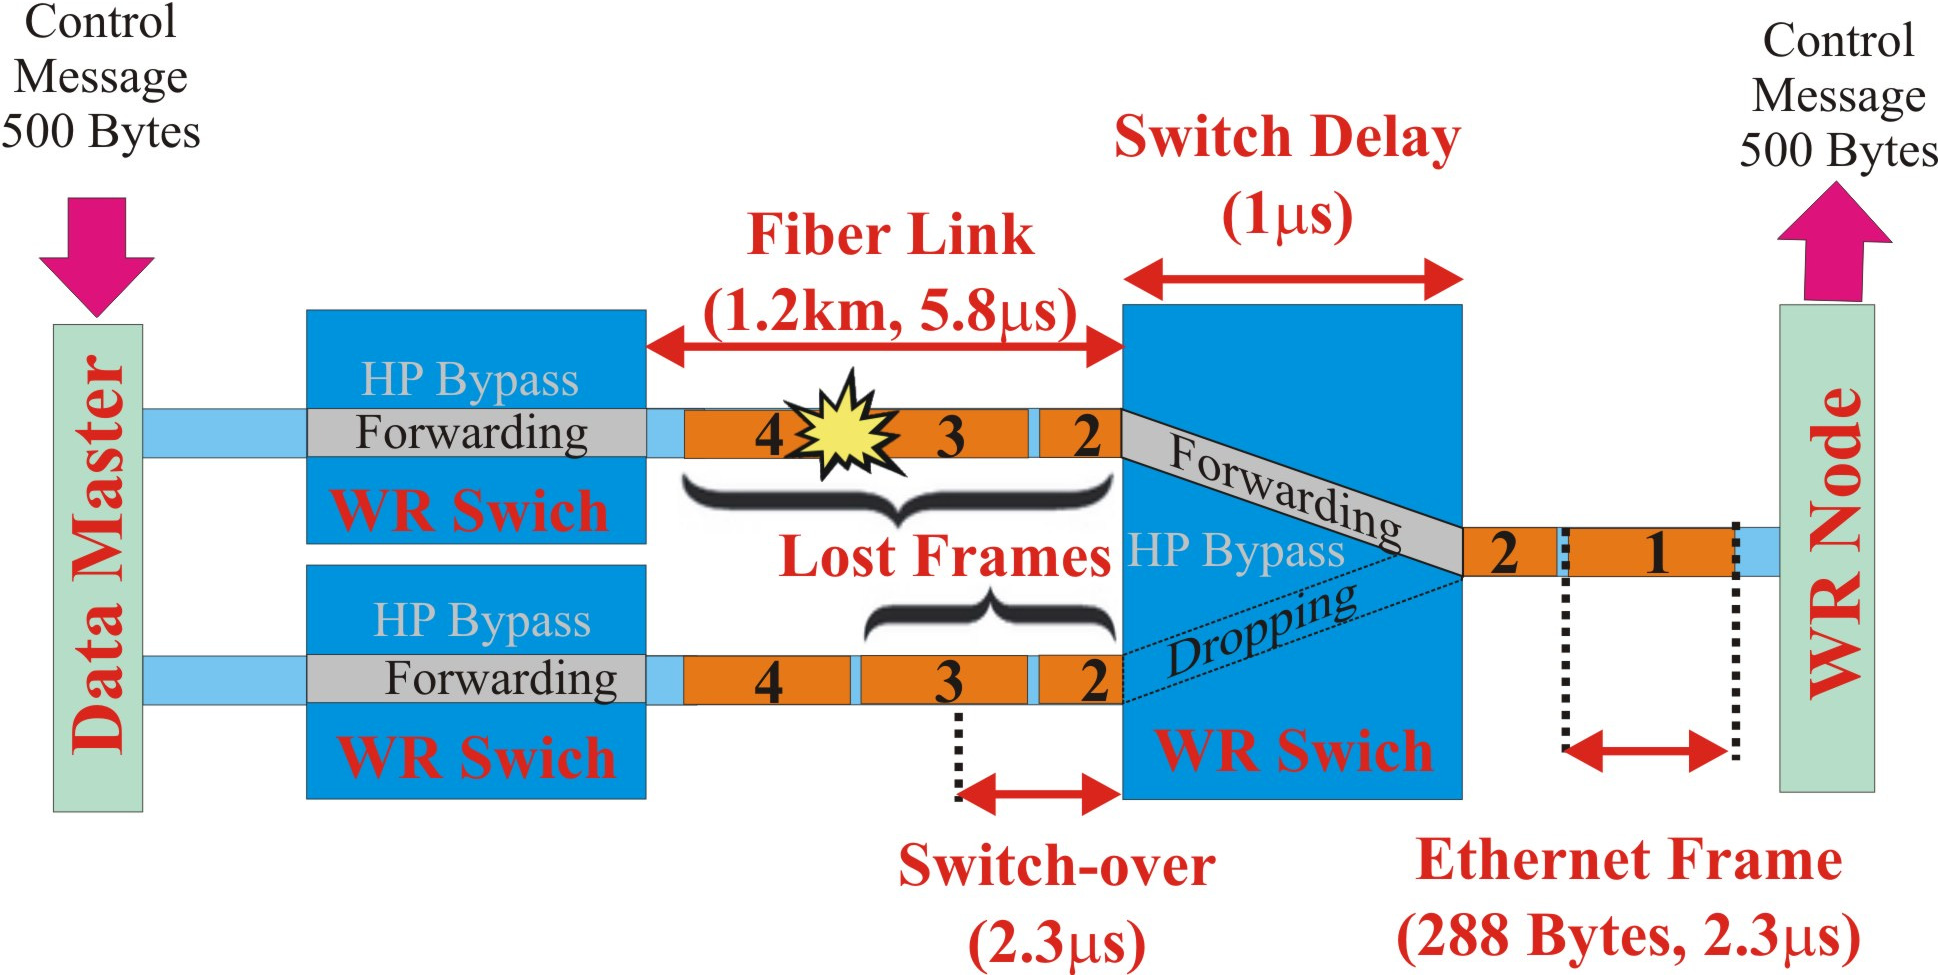
\includegraphics[height=5cm,keepaspectratio]{robustness/RSTPsimple.ps}

\end{frame}
%%%%%%%%%%%%%%%%%%%%%%%%%%%%%%%%%%%%%%%%%%%%%%%%%%%%%%%%%%%%%%%%%%%%%%%%%%%%%%
\begin{frame}
  \frametitle{WR RSTP -- real-life consideration}   
%%%%%%%%%%%%%%%%%%%%%%%%%%%%%%%%%%%%%%%%%%%%%%%%%%%%%%%%%%%%%%%%%%%%%%%%%%%%%%

\centering
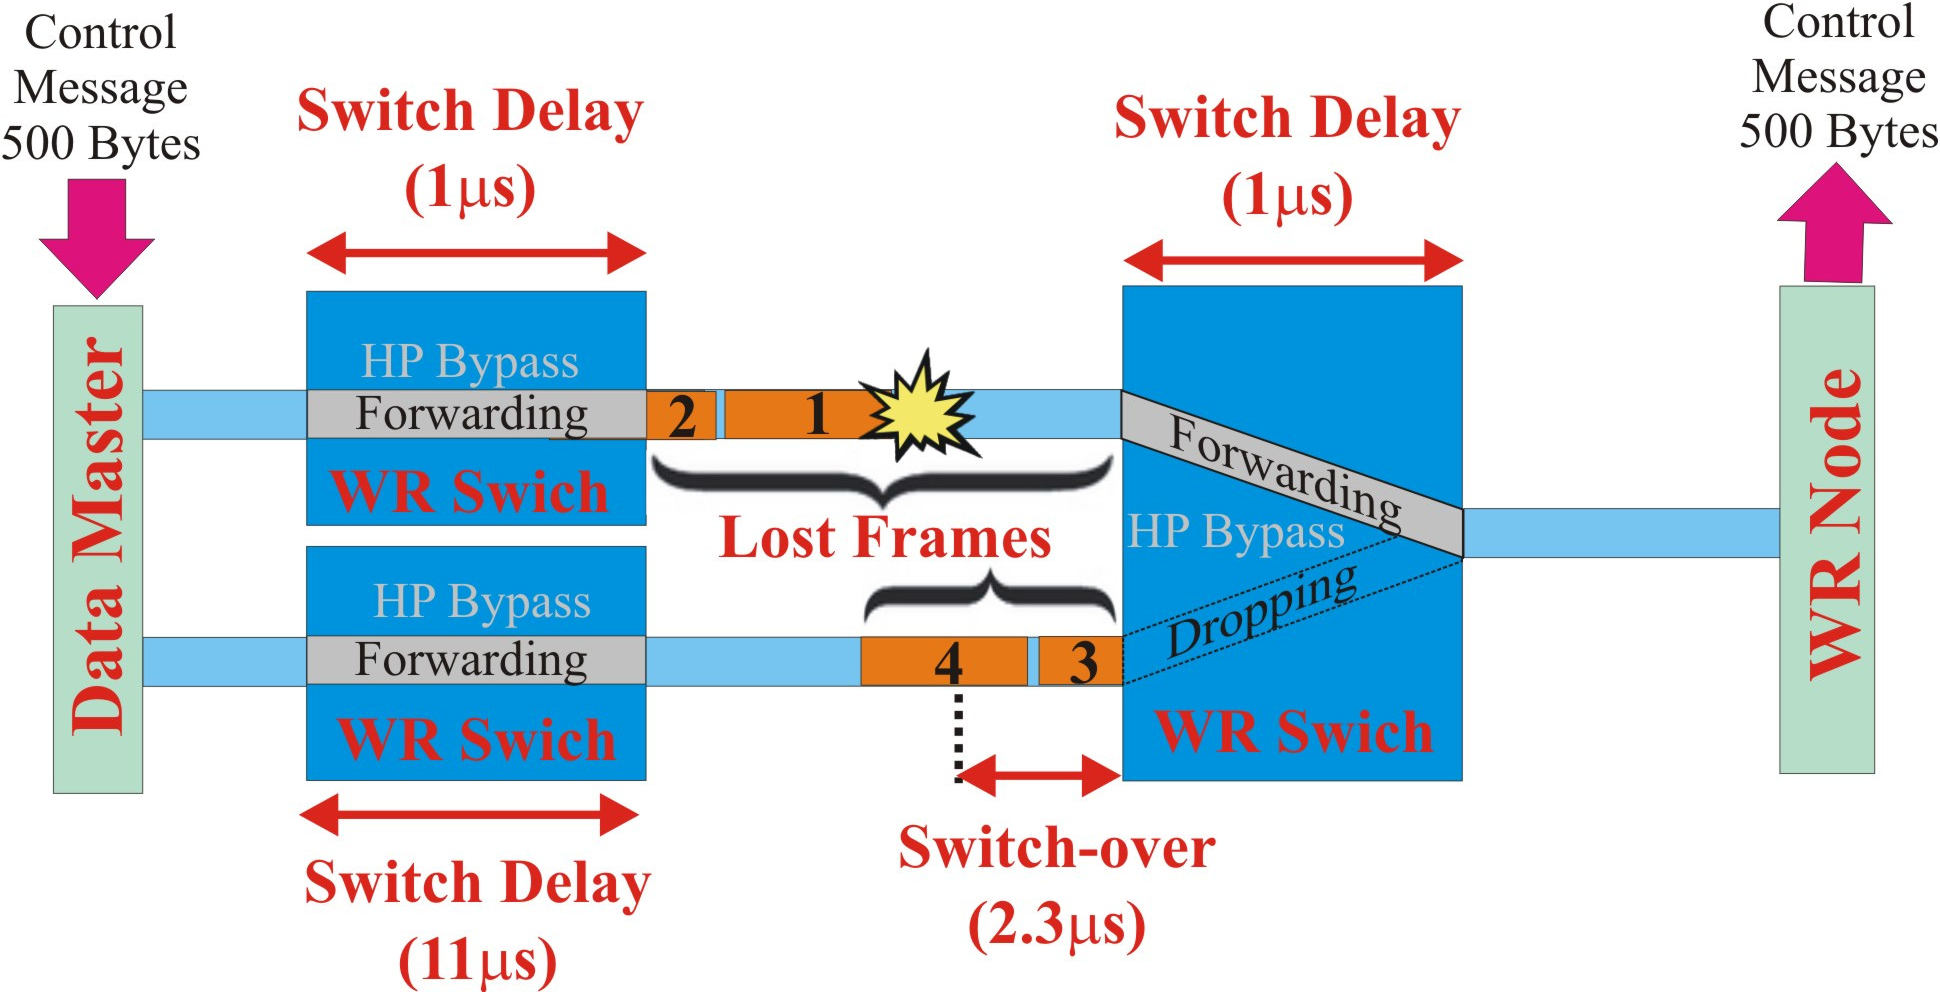
\includegraphics[height=5cm,keepaspectratio]{robustness/RSTPcomplex2.ps}

  \begin{itemize}
    \item Introducing maximum cut-through delay (13$us$) on backup ports of the
          switch.
    \item Backup link always 1 hoop longer then active.
  \end{itemize}

\end{frame}
%%%%%%%%%%%%%%%%%%%%%%%%%%%%%%%%%%%%%%%%%%%%%%%%%%%%%%%%%%%%%%%%%%%%%%%%%%%%%%
\begin{frame}
  \frametitle{Data Redundancy (FEC)}   
%%%%%%%%%%%%%%%%%%%%%%%%%%%%%%%%%%%%%%%%%%%%%%%%%%%%%%%%%%%%%%%%%%%%%%%%%%%%%%

      \begin{itemize}
      \item Reed-Solomon for package-based encoding:
	\begin{itemize}
	\item  4 Ethernet Frames (2 x original, 2 x parity) for input of size 
	      $<\approx2500$. We can lose any 2 packages (out of 4).
	\item  ????? for $>\approx2500$
	\end{itemize}
      \item Hamming for bit-based encoding -- Single Error Detection-Double
	    Error Correction (SEC-DED).
      \item FEC needs to know the size of incoming CM at the beginning of the
	  encoding (needs to be provided in non-standard way, i.e. user defined
	  register, WB address 0x2)
      \end{itemize}

\centering
\textcolor{red}{DISCUSSION:} \\
{\small
How do we want to transfer CM $>$ 1500Bytes (i.e. 5000Bytes)? Burst?
non-standard size of the payload? \\
How do we indicate that FEC is to be used? EtherType? WB special reg? 
}
\end{frame}

%%%%%%%%%%%%%%%%%%%%%%%%%%%%%%%%%%%%%%%%%%%%%%%%%%%%%%%%%%%%%%%%%%%%%%%%%%%%%%
\begin{frame}
  \frametitle{Flow and Congestion Control }
%%%%%%%%%%%%%%%%%%%%%%%%%%%%%%%%%%%%%%%%%%%%%%%%%%%%%%%%%%%%%%%%%%%%%%%%%%%%%%
\centering
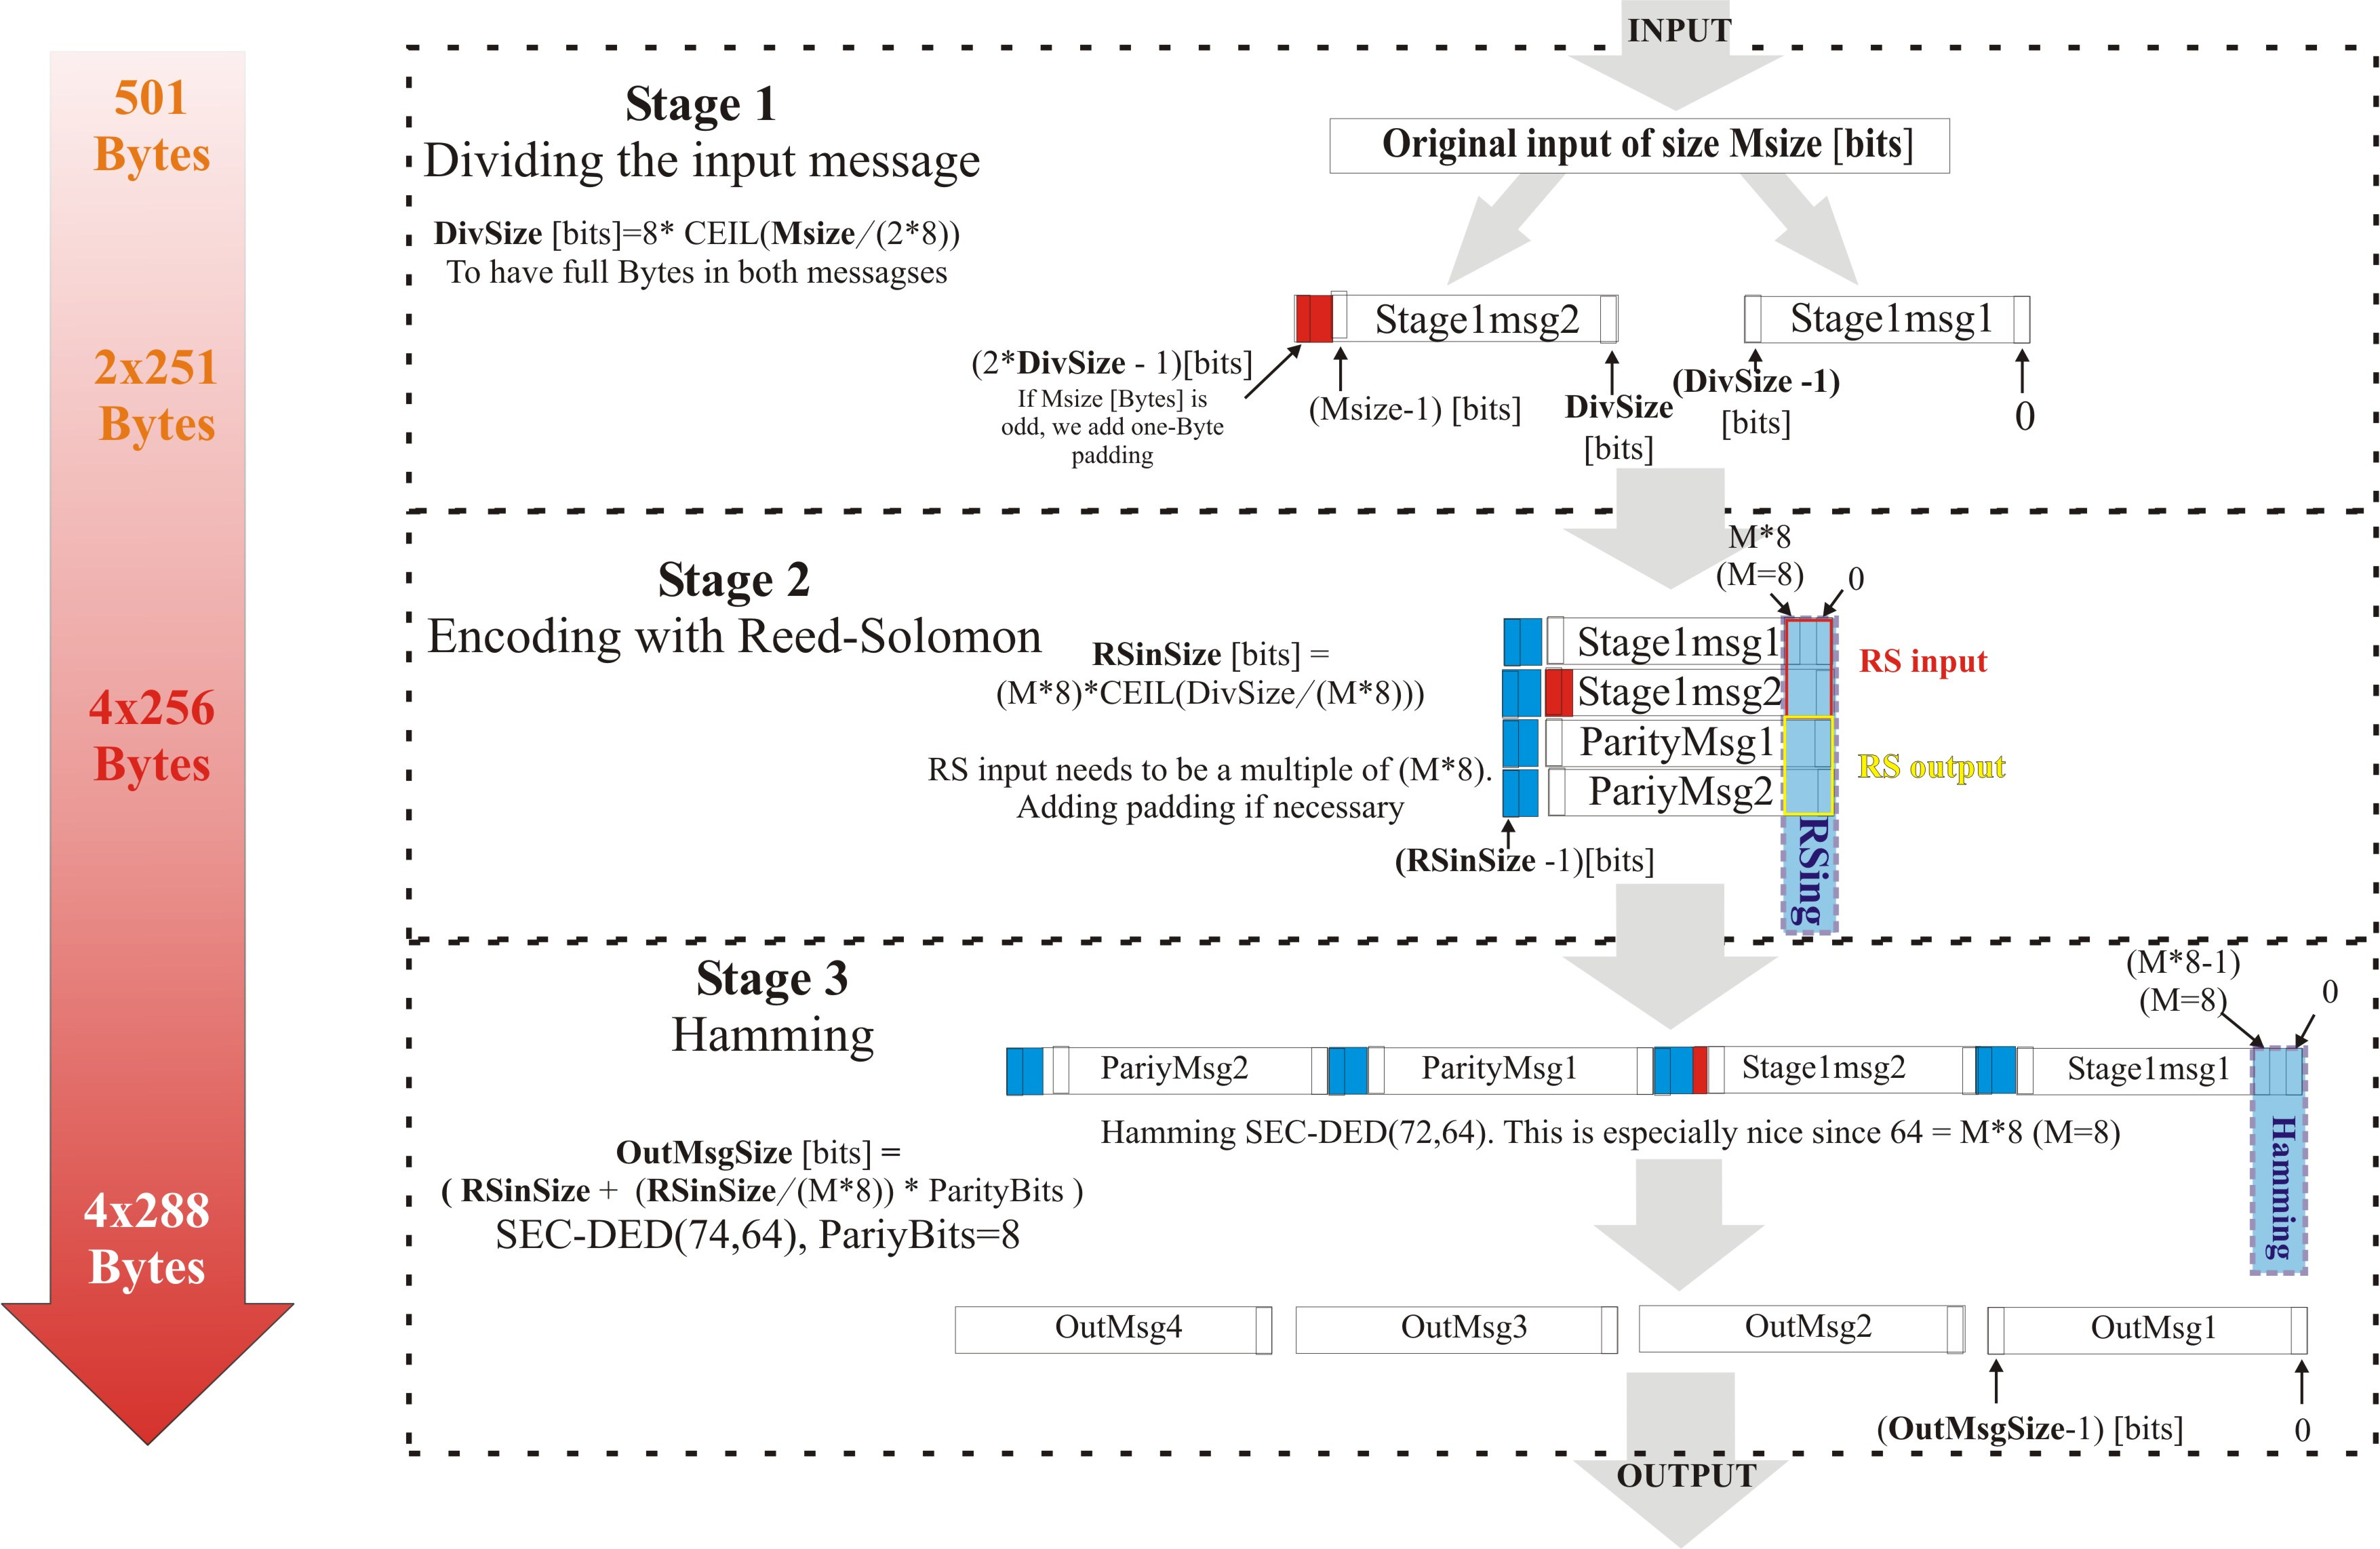
\includegraphics[height=7cm,keepaspectratio]{robustness/FECflow.ps}

\end{frame}


%%%%%%%%%%%%%%%%%%%%%%%%%%%%%%%%%%%%%%%%%%%%%%%%%%%%%%%%%%%%%%%%%%%%%%%%%%%%%%
\begin{frame}
  \frametitle{Flow and Congestion Control}   
%%%%%%%%%%%%%%%%%%%%%%%%%%%%%%%%%%%%%%%%%%%%%%%%%%%%%%%%%%%%%%%%%%%%%%%%%%%%%%

\textcolor{blue}{Cesars playground: blocking of HP traffic from other ports then
Data Master}
\centering
\textcolor{red}{DISCUSSION:} 

\end{frame}

%%%%%%%%%%%%%%%%%%%%%%%%%%%%%%%%%%%%%%%%%%%%%%%%%%%%%%%%%%%%%%%%%%%%%%%%%%%%%%
\subsection{Monitoring and Diagnostics}
\begin{frame}
  \frametitle{Monitoring and Diagnostics of WR-specific parameters}   
%%%%%%%%%%%%%%%%%%%%%%%%%%%%%%%%%%%%%%%%%%%%%%%%%%%%%%%%%%%%%%%%%%%%%%%%%%%%%%

Cesar's playground...
\begin{itemize}
 \item Detection of lost HP Frames (in WR Switches) using FEC ID and CM ID
      (stored in the header added by FEC).
 \item Precise knowledge of HP traffic delays on the path DataMaster $<->$ Node.
 \item Monitoring of WRPTP parameters.
\end{itemize}
\centering
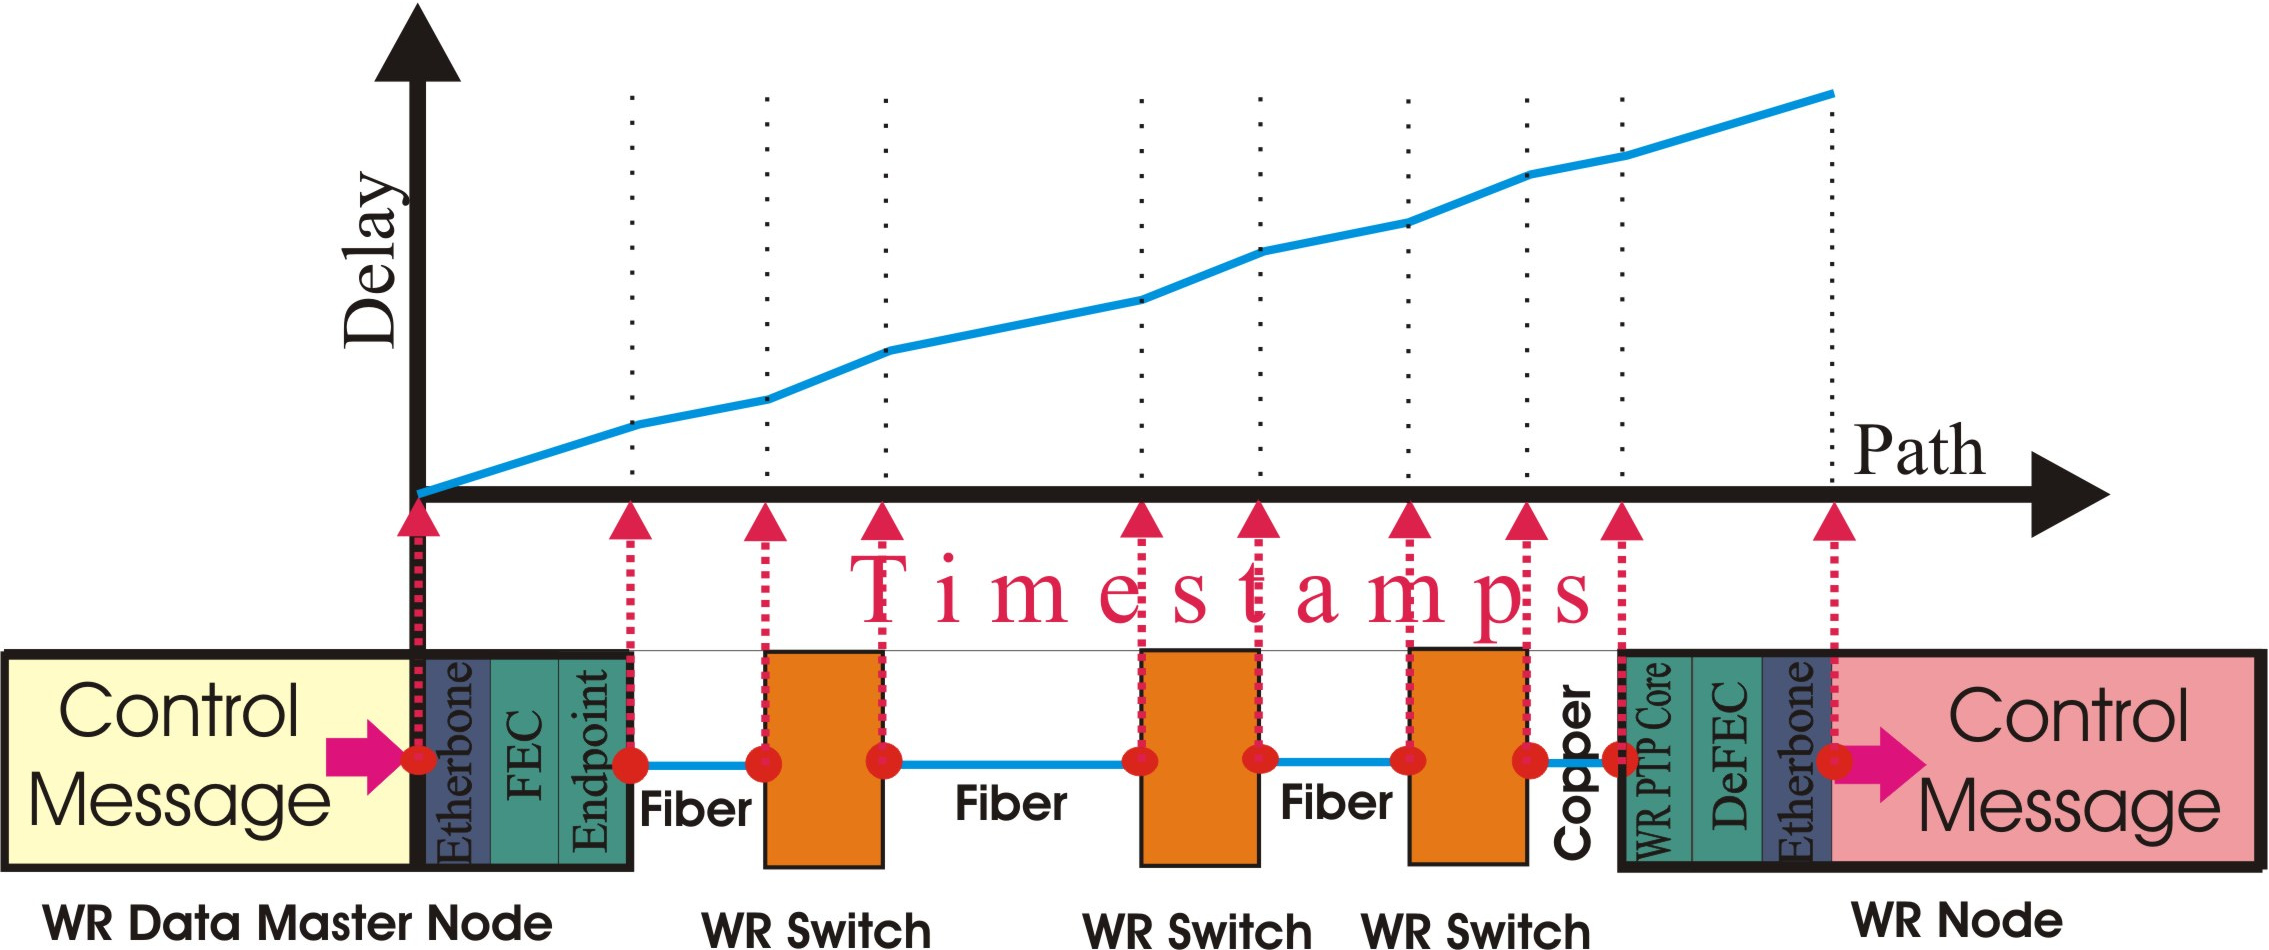
\includegraphics[height=4cm,keepaspectratio]{robustness/delayMonitoring.ps}

\end{frame}

%%%%%%%%%%%%%%%%%%%%%%%%%%%%%%%%%%%%%%%%%%%%%%%%%%%%%%%%%%%%%%%%%%%%%%%%%%%%%%
\section{DISCUSSION (OHMG)}
\subsection{Oh, My God !!!}
\begin{frame}
  \frametitle{Summary of issues to be discussed}   
%%%%%%%%%%%%%%%%%%%%%%%%%%%%%%%%%%%%%%%%%%%%%%%%%%%%%%%%%%%%%%%%%%%%%%%%%%%%%%

  \begin{columns}[c]
  \column{2.5in}  % slides are 3in high by 5in wide
{\footnotesize 
  \begin{itemize}
  \item \textbf{Naming}: Granularity Window, High Priority, Standard Priority,
        Control Messages.
  \item \textbf{Requirements}: 
  {\footnotesize 
  \begin{itemize}
    \item What is the real-life requirement for number of CM lost per year?
    \item GW of 100$\mu s$ is very tight and needs solid justification.
  \end{itemize}
  }
  \item \textbf{Cut-through Bypass}: Drop on collision, sending of HP traffic by
        more Data Master and/or nodes.
  \item \textbf{Topology Redundancy}: Redundant connection to WR nodes.
  \end{itemize}
}
  \column{2.5in}
  {\footnotesize 
  \begin{itemize}
  \item \textbf{RSTP}:Ring topology - impossible with current approach, is it
        worth considering, what is the feasibility of ring WRN?.
  \item \textbf{Data Redundancy (FEC)}:
  {\footnotesize 
      \begin{itemize}
      \item how do we want to transfer CM $>$ 1500 Bytes (i.e. 5000 Bytes)?
            Burst? non standard size payload?
      \item How do we indicate that FEC is to be used? EtherType? Special WB
	    register (addr=0x2)? 
      \end{itemize}
  }
  \item \textbf{Flow and Congestion Control }:
  \item \textbf{Monitoring and Diagnostics of WR-specific parameters}:
  \end{itemize}
}
  \end{columns}


\end{frame}


\end{document}
